\documentclass{standalone}

\usepackage{tikz}
\usetikzlibrary{backgrounds, calc, intersections, through}

\begin{document}

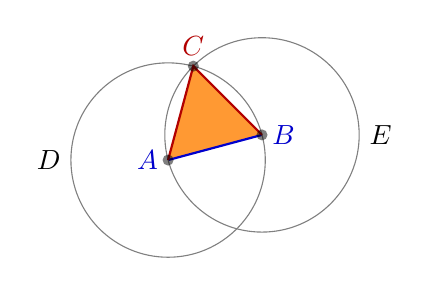
\begin{tikzpicture}[thick,help lines/.style={thin,draw=black!50}]
  \def\A{\textcolor{input}{$A$}}     \def\B{\textcolor{input}{$B$}}
  \def\C{\textcolor{output}{$C$}}    \def\D{$D$}
  \def\E{$E$}

  \colorlet{input}{blue!80!black}    \colorlet{output}{red!70!black}
  \colorlet{triangle}{orange}

  \coordinate [label=left:\A]  (A) at ($ (0,0) + .1*(rand,rand) $);
  \coordinate [label=right:\B] (B) at ($ (1.25,0.25) + .1*(rand,rand) $);

  \draw [input] (A) -- (B);

  \node [name path=D,help lines,draw,label=left:\D]   (D) at (A) [circle through=(B)] {};
  \node [name path=E,help lines,draw,label=right:\E]  (E) at (B) [circle through=(A)] {};

  \path [name intersections={of=D and E,by={[label=above:\C]C}}];

  \draw [output] (A) -- (C) -- (B);

  \foreach \point in {A,B,C}
  \fill [black,opacity=.5] (\point) circle (2pt);

  \begin{pgfonlayer}{background}
    \fill[triangle!80] (A) -- (C) -- (B) -- cycle;
  \end{pgfonlayer}
\end{tikzpicture}

\end{document}
